\documentclass[11pt]{article}
\usepackage{hyperref}
\usepackage{amsthm}
\usepackage{amsmath}
\usepackage{amsfonts}
\usepackage{tikz}
\usepackage{ wasysym }
\usepackage{fancyvrb}
\usetikzlibrary{arrows.meta,positioning}


\newtheorem{example}{Example}


\author{Group 1:  David Garza,  Garrison Kleman, Nicholas Jacob, Hannah Jensen}
\title{Homework 3 Advanced Analytics and Metaheuristics}

\begin{document}
\maketitle

\begin{enumerate}
\item Team Building
\begin{enumerate}
\item 
\item
\end{enumerate}
\item Outdoor Grilling

Below is our model diagram.  

 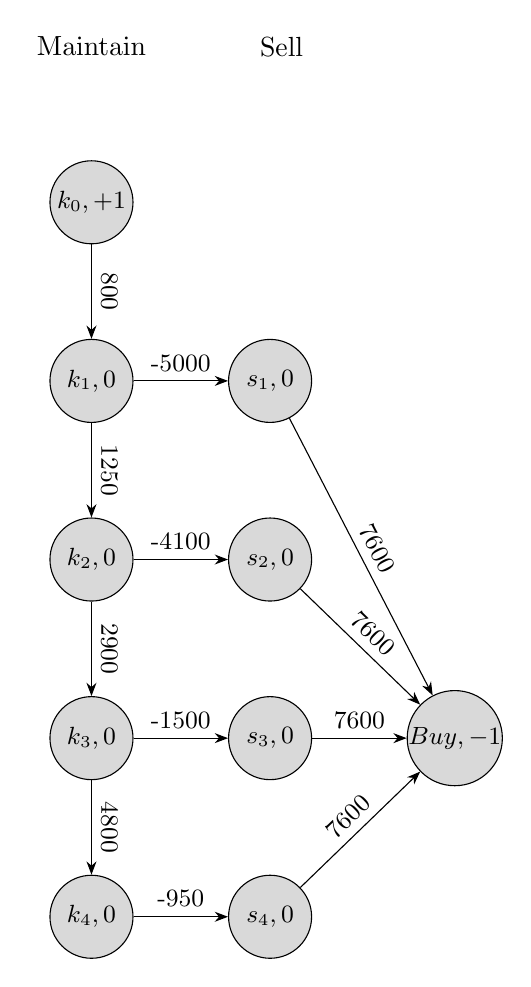
\begin{tikzpicture}[
      mycircle/.style={
         circle,
         draw=black,
         fill=gray,
         fill opacity = 0.3,
         text opacity=1,
         inner sep=0pt,
         minimum size=30pt,
         font=\small},
      myarrow/.style={-Stealth},
      node distance=1.2cm and 1.2cm
      ]
      \node[mycircle] (k0) {$k_0, +1$};
      \node[mycircle,below =of k0] (k1) {$k_1, 0$};
      \node[mycircle,below=of k1] (k2) {$k_2, 0$};
	 \node[mycircle,below=of k2] (k3) {$k_3, 0$};
	 \node[mycircle,below=of k3] (k4) {$k_4, 0$};
	 \node[mycircle,right=of k1] (s1) {$s_1, 0$};
	 \node[mycircle,below=of s1] (s2) {$s_2, 0$};
	\node[mycircle,below=of s2] (s3) {$s_3, 0$};
	\node[mycircle,below=of s3] (s4) {$s_4, 0$};
	%\node[mycircle,below=of s4] (s5) {$s_5, 0$};
	
	 \node[above = of k0](text){Maintain};
      \node[right = of text] {Sell};

      \node[mycircle,right=of s3] (buynew) {$Buy, -1$};

    \foreach \i/\j/\txt/\p in {% start node/end node/text/position
      k0/k1/800/above,
      k1/k2/1250/above,
      k2/k3/2900/above,
      k3/k4/4800/above,
      k1/s1/-5000/above,
      k2/s2/-4100/above,
      k3/s3/-1500/above,
      k4/s4/-950/above,
      %k4/s5/0/above,
	 s1/buynew/7600/above,
	 s2/buynew/7600/above,
	 s3/buynew/7600/above,
	 s4/buynew/7600/above}
	 %s5/buynew/7600/above}
       \draw [myarrow] (\i) -- node[sloped,font=\small,\p] {\txt} (\j);


    \end{tikzpicture}

Here is our model file:

{\small \VerbatimInput{group1_HW3_p2.mod}}

Here is our data file:

{\small \VerbatimInput{group1_HW3_p2.dat}}

Here is our output:

%\includegraphics[width = .9\textwidth]{output_p2.png}

\item Race Car Tires

 Here is my flow model:  All nodes have zero $b$ costs are displayed on arcs.  If minimums are needed, the ordered triple represents $(cost,lowerLimit,upperLimit)$.  The $v$ nodes are virtual to balance the flow.


 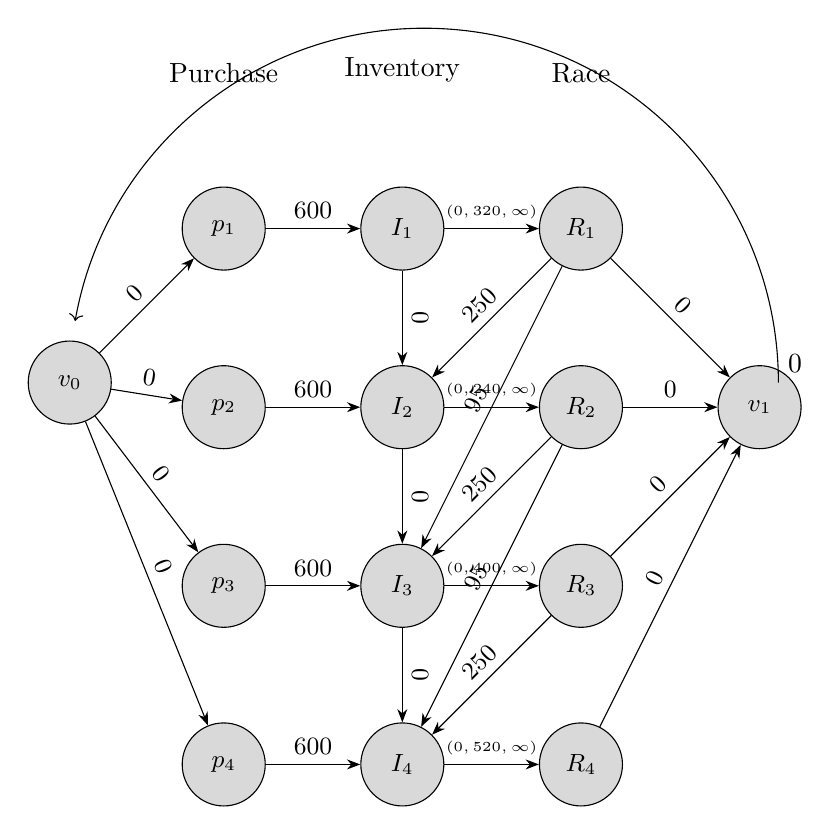
\begin{tikzpicture}[
      mycircle/.style={
         circle,
         draw=black,
         fill=gray,
         fill opacity = 0.3,
         text opacity=1,
         inner sep=0pt,
         minimum size=30pt,
         font=\small},
      myarrow/.style={-Stealth},
      node distance=1.2cm and 1.2cm
      ]
      \node[mycircle] (v0){$v_0$};
      \node[mycircle,above right =of v0] (p1){$p_1$};
      \node[mycircle,below=of p1] (p2) {$p_2$};
	 \node[mycircle,below=of p2] (p3) {$p_3$};
	 \node[mycircle,below=of p3] (p4) {$p_4$};
      \node[mycircle,right=of p1] (i1) {$I_1$};
      \node[mycircle,below=of i1] (i2) {$I_2$};
	 \node[mycircle,below=of i2] (i3) {$I_3$};
	 \node[mycircle,below=of i3] (i4) {$I_4$};
      \node[mycircle,right=of i1] (r1) {$R_1$};
      \node[mycircle,below=of r1] (r2) {$R_2$};
	 \node[mycircle,below=of r2] (r3) {$R_3$};
	 \node[mycircle,below=of r3] (r4) {$R_4$};      
      \node[mycircle,right=of r2] (v1) {$v_1$};
      
      \node[above = of p1] (p) {Purchase};
      \node[above = of i1] (i) {Inventory};
      \node[above = of r1] (r) {Race};




    \foreach \i/\j/\txt/\p in {% start node/end node/text/position
      v0/p1/0/above,
	 v0/p2/0/above,
      v0/p3/0/above,
	 v0/p4/0/above,
      p1/i1/600/above,
      p2/i2/600/above,
      p3/i3/600/above,
      p4/i4/600/above,
	r1/i2/250/above,
	r1/i3/95/above,
	r2/i3/250/above,
	r2/i4/95/above,
	r3/i4/250/above,
	r1/v1/0/above,
	r2/v1/0/above,
	r3/v1/0/above,
	r4/v1/0/above,
	i1/i2/0/above,
	i2/i3/0/above,
	i3/i4/0/above}
       \draw [myarrow] (\i) -- node[sloped,font=\small,\p] {\txt} (\j);

	\draw[myarrow] (i1) -- node[sloped, font = \tiny, above] {$(0,320,\infty)$} (r1);
\draw[myarrow] (i2) -- node[sloped, font = \tiny, above] {$(0,240,\infty)$} (r2);
\draw[myarrow] (i3) -- node[sloped, font = \tiny, above] {$(0,400,\infty)$} (r3);
\draw[myarrow] (i4) -- node[sloped, font = \tiny, above] {$(0,520,\infty)$} (r4);

	\draw[->] (9,0) node[above right,style={-Stealth}]{0} arc  (0:170:4.5) ;

    \end{tikzpicture}

Here is our model file:

{\small \VerbatimInput{group1_HW3_p3.mod}}

Here is our data file:

{\small \VerbatimInput{group1_HW3_p3.dat}}

Here is our output:

\includegraphics[width = .9\textwidth]{output_p3.png}

We look to be purchasing new tires for both the needs of the first two races, 320 and 200 respectively.  This is the maximum number of tires needed.  We use the normal service on 280 tires from the first race and quick on the other 40.  In second race we use the normal service on 120 but quick fix 120.  For the third race we quick fix all 400 tires used.  We end up with exactly the number of tires needed in the fourth race.  Total cost is \$490 000.

\item Dunder Mifflin

By far our most complicated model.  Unhired workers will flow to the worker pool, $wp$ and flow back out to the Workers with a weight of zero to maintain the flow.  $g$ and $s$ represent the available generalist and specialists.  If they are hired, they flow to the hired pool of each type.  They are then transported to each plant at the respective cost.  We then convert each worker into their number of products created with the weight.  Finally we combine the number of possible products they can create into each location.  Inventory is created with the regular cost but with limits on the maximums.  Overtime is represented in red and uses a different virtual node for each location.  Inventory is then shipped from each of the factories to the different businesses we serve, meeting the demand as represented inside the node.  We attempted to make the flow circular but do to the difference in weights based on employment categories, could never get it to create a balanced flow.

This model provides labor for overtime but does not account for a premium the wage for the employee working outside of regular hours.  We see this as an assumption that there is not a bump in pay for working second shift but there is a 50\% increase in our overhead costs of production.

 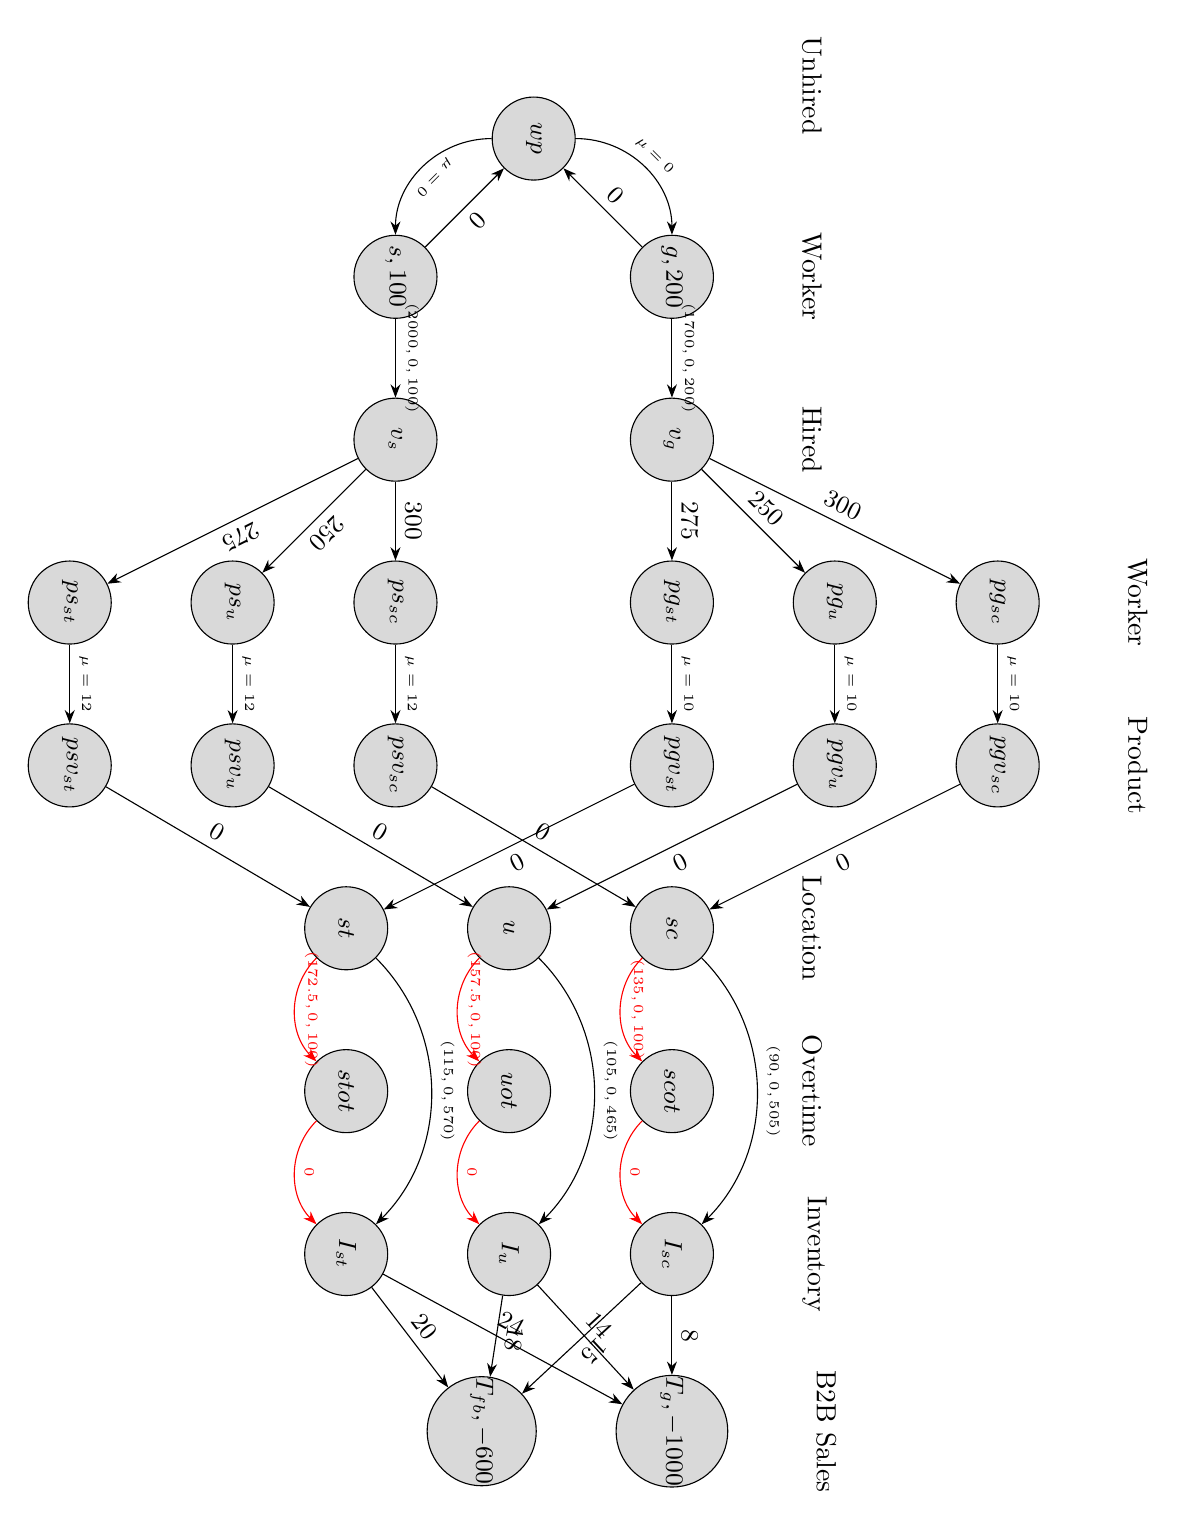
\begin{tikzpicture}[rotate=270,transform shape,
      mycircle/.style={
         circle,
         draw=black,
         fill=gray,
         fill opacity = 0.3,
         text opacity=1,
         inner sep=0pt,
         minimum size=30pt,
         font=\small},
      myarrow/.style={-Stealth},
      node distance=1.0cm and 1.0cm
      ]
      \node[mycircle] (v0){$wp$};
      \node[mycircle,above right=of v0] (g){$g, 200$};
      \node[mycircle,below right=of v0] (s){$s, 100$};
      \node[mycircle, right =of g] (vg){$v_g$};
      \node[mycircle, right =of s] (vs){$v_s$};
      \node[mycircle, right =of vg] (pgst){$pg_{st}$};
	\node[mycircle, above =of pgst] (pgu){$pg_u$};
      \node[mycircle, above =of pgu] (pgsc){$pg_{sc}$};	 
      \node[mycircle, right =of vs] (pssc){$ps_{sc}$};
      \node[mycircle, below =of pssc] (psu){$ps_{u}$};
      \node[mycircle, below =of psu] (psst){$ps_{st}$};	
      \node[mycircle, right =of pgsc] (pgvsc){$pgv_{sc}$};
      \node[mycircle, right =of pgu] (pgvu){$pgv_{u}$};
      \node[mycircle, right =of pgst] (pgvst){$pgv_{st}$};
      \node[mycircle, right =of pssc] (psvsc){$psv_{sc}$};
      \node[mycircle, right =of psu] (psvu){$psv_{u}$};
      \node[mycircle, right =of psst] (psvst){$psv_{st}$};

      \node[mycircle, right =of pgvst] (sc){$sc$};
      \node[mycircle, below =of sc] (u){$u$};
      \node[mycircle, below =of u] (st){$st$};

	\node[mycircle, right = of sc] (scot) {$scot$};
      \node[mycircle, below =of scot] (uot){$uot$};
      \node[mycircle, below =of uot] (stot){$stot$};

	  \node[mycircle, right =of scot] (isc){$I_{sc}$};
      \node[mycircle, below =of isc] (iu){$I_u$};
      \node[mycircle, below =of iu] (ist){$I_{st}$};

	  \node[mycircle, right =of isc] (tg){$T_{g}, -1000$};
      \node[mycircle, below =of tg] (tfb){$T_{fb}, -600$};

\node[above = of pgsc] (workers){Worker};
\node[above = of pgvsc] (wtoprod){Product};
\node[above = of sc] (loc){Location};
\node[above = of scot](ot){Overtime};
\node[above = of isc](inventory){Inventory};
\node[above = of tg]{B2B Sales};
\node[above = of vg]{Hired};
\node[above = of g](w){Worker};
\node[left = of w]{Unhired};

	  %\node[mycircle, right =of tg] (dg){$D_{g},-1000$};
      %\node[mycircle, below =of dg] (dfb){$D_{fb},-600$};

      %\node[mycircle, below right =of dg] (v1){$v_{1}$};


    \foreach \i/\j/\txt/\p in {% start node/end node/text/position
      g/v0/0/above,
	  s/v0/0/above,
	 vg/pgsc/300/above,
	vg/pgu/250/above,
	vg/pgst/275/above,
	 vs/pssc/300/above,
	vs/psu/250/above,
	vs/psst/275/above,
	pgvsc/sc/0/above,
	psvsc/sc/0/above,
	pgvu/u/0/above,
	psvu/u/0/above,
	pgvst/st/0/above,
	psvst/st/0/above,
isc/tg/8/above,
isc/tfb/15/above,
iu/tg/14/above,
iu/tfb/18/above,
ist/tg/24/above,
ist/tfb/20/above}
       \draw [myarrow] (\i) -- node[sloped,font=\small,\p] {\txt} (\j);

%\draw[->] (18,-1) node[above right,style={-Stealth}]{0} arc  (0:170:9.0) ;


\draw[myarrow] (g) -- node[sloped, font = \tiny, above] {$(1700,0,200)$} (vg);
\draw[myarrow] (s) -- node[sloped, font = \tiny, above] {$(2000,0,100)$} (vs);
\draw[myarrow] (pgsc) -- node[sloped, font = \tiny, above] {$\mu = 10$} (pgvsc);
\draw[myarrow] (pgu) -- node[sloped, font = \tiny, above] {$\mu = 10$} (pgvu);
\draw[myarrow] (pgst) -- node[sloped, font = \tiny, above] {$\mu = 10$} (pgvst);
\draw[myarrow] (pssc) -- node[sloped, font = \tiny, above] {$\mu = 12$} (psvsc);
\draw[myarrow] (psu) -- node[sloped, font = \tiny, above] {$\mu = 12$} (psvu);
\draw[myarrow] (psst) -- node[sloped, font = \tiny, above] {$\mu = 12$} (psvst);

\draw[myarrow] (sc) to [out = 45, in=135] node[sloped, font = \tiny, above] {$(90,0,505)$} (isc);
\draw[myarrow] (u) to [out = 45, in=135] node[sloped, font = \tiny, above] {$(105,0,465)$} (iu);
\draw[myarrow] (st) to [out = 45, in=135] node[sloped, font = \tiny, above] {$(115,0,570)$} (ist);
\draw[myarrow,red] (sc) to [out = -45, in=-135] node[sloped, font = \tiny, above] {$(135,0,100)$} (scot);
\draw[myarrow,red] (u) to [out = -45, in=-135] node[sloped, font = \tiny, above] {$(157.5,0,100)$} (uot);
\draw[myarrow,red] (st) to [out = -45, in=-135] node[sloped, font = \tiny, above] {$(172.5,0,100)$} (stot);
\draw[myarrow,red] (scot) to [out = -45, in=-135] node[sloped, font = \tiny, above] {$0$} (isc);
\draw[myarrow,red] (uot) to [out = -45, in=-135] node[sloped, font = \tiny, above] {$0$} (iu);
\draw[myarrow,red] (stot) to [out = -45, in=-135] node[sloped, font = \tiny, above] {$0$} (ist);

\draw[myarrow] (v0) to [out = 90, in=180] node[sloped, font = \tiny, above] {$\mu = 0$} (g);
\draw[myarrow] (v0) to [out = 270, in=180] node[sloped, font = \tiny, above] {$\mu = 0$} (s);

%\draw[myarrow] (tg) -- node[sloped, font = \tiny, above] {$(0,1000,\infty)$} (dg);
%\draw[myarrow] (tfb) -- node[sloped, font = \tiny, above] {$(0,600,\infty)$} (dfb);
    \end{tikzpicture}
Here is our model file:

{\tiny \VerbatimInput{group1_HW3_p4.mod}}

Here is our data file:

{\tiny \VerbatimInput{group1_HW3_p4.dat}}

Here is my output:

\includegraphics[width = .9\textwidth]{output_p4.png}

Solution is non-integer in employees which is unfortunate but can be the case with the generalized network flow problems.  All 100 specialists are hired, 40 generalists.  Scranton does use 60 products of OT, none of the other plants do but they max out production at each.

\item Mud b Gone

 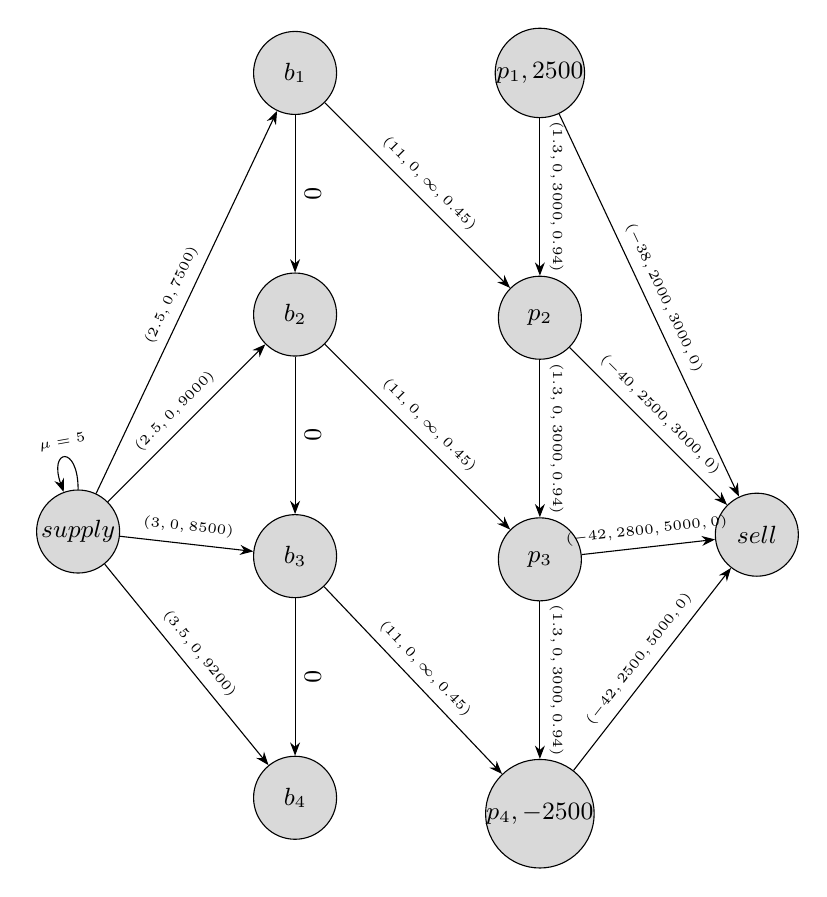
\begin{tikzpicture}[transform shape,
      mycircle/.style={
         circle,
         draw=black,
         fill=gray,
         fill opacity = 0.3,
         text opacity=1,
         inner sep=0pt,
         minimum size=30pt,
         font=\small},
      myarrow/.style={-Stealth},
      node distance=2cm and 2cm
      ]
      \node[mycircle] (b1){$b_1$};
      \node[mycircle, below = of b1] (b2){$b_2$};
      \node[mycircle, below = of b2] (b3){$b_3$};
      \node[mycircle, below = of b3] (b4){$b_4$};


      \node[mycircle, right = of b1] (p1){$p_1,2500$};
      \node[mycircle, below = of p1] (p2){$p_2$};
      \node[mycircle, below = of p2] (p3){$p_3$};
      \node[mycircle, below = of p3] (p4){$p_4,-2500$};


      \node[mycircle, below right = of p2] (sell){$sell$};
      \node[mycircle, below left = of b2] (supply){$supply$};


    \foreach \i/\j/\txt/\p in {% start node/end node/text/position
	  b1/b2/0/above,
	b2/b3/0/above,
	b3/b4/0/above}
       \draw [myarrow] (\i) -- node[sloped,font=\small,\p] {\txt} (\j);

\draw[myarrow] (supply) -- node[sloped, font = \tiny, above] {$(2.5,0,7500)$} (b1);
\draw[myarrow] (supply) -- node[sloped, font = \tiny, above] {$(2.5,0,9000)$} (b2);
\draw[myarrow] (supply) -- node[sloped, font = \tiny, above] {$(3,0,8500)$} (b3);
\draw[myarrow] (supply) -- node[sloped, font = \tiny, above] {$(3.5,0,9200)$} (b4);
%
\draw[myarrow] (p1) -- node[sloped, font = \tiny, above] {$(-38,2000,3000,0)$} (sell);
\draw[myarrow] (p2) -- node[sloped, font = \tiny, above] {$(-40,2500,3000,0)$} (sell);
\draw[myarrow] (p3) -- node[sloped, font = \tiny, above] {$(-42,2800,5000,0)$} (sell);
\draw[myarrow] (p4) -- node[sloped, font = \tiny, above] {$(-42,2500,5000,0)$} (sell);
%
\draw[myarrow] (p1) -- node[sloped, font = \tiny, above] {$(1.3,0,3000,0.94)$} (p2);
\draw[myarrow] (p2) -- node[sloped, font = \tiny, above] {$(1.3,0,3000,0.94)$} (p3);
\draw[myarrow] (p3) -- node[sloped, font = \tiny, above] {$(1.3,0,3000,0.94)$} (p4);
%
\draw[myarrow] (b1) -- node[sloped, font = \tiny, above] {$(11,0,\infty,0.45)$} (p2);
\draw[myarrow] (b2) -- node[sloped, font = \tiny, above] {$(11,0,\infty,0.45)$} (p3);
\draw[myarrow] (b3) -- node[sloped, font = \tiny, above] {$(11,0,\infty,0.45)$} (p4);
%
\draw[myarrow] (supply) to [out = 90, in=110, looseness = 8] node[sloped, font = \tiny, above] {$\mu = 5$} (supply);


    \end{tikzpicture}

Here is our model file:

{\tiny\VerbatimInput{group1_HW3_p5.mod}}

Here is our data file:

{\tiny \VerbatimInput{group1_HW3_p5.dat}}

\begin{enumerate}
\item We see a solution for our flow.  We sell 2000, 2500, 4220 and 2500 in each of the respective periods.  We remark on the infinite supply house obtained by creating a loop with a $\mu$ factor set to 5 but could be any value greater than 1.

\includegraphics[width = .9\textwidth]{output_p5a.png}
\item We next look at sensitivity of the capacity.  We see a value of -\$5.40 in the report, supply to b2.  We interpret this as having additional gallons of base will increase (recall minimizing) our income by \$5.40.  Both the up and the down are reported as 0.  We are unsure of how to interpret this as we clearly would use more of the base if it was available but are unsure why these values are all zero.  We even broke apart the upper and lower limit thinking this was the issue but did not change the up and down on the shadow price.  We do clearly see this as the bottle neck in our model.

\includegraphics[width = .9\textwidth]{output_p5b.png}
\item We see that the contribution to the cost is -\$40 on the flow from p2 to Sold.  This value can be modified up to -\$42 and not change the model at all.  


\includegraphics[width = .9\textwidth]{output_p5c.png}
\end{enumerate}

\end{enumerate}



\end{document}
